

\tikzset{every picture/.style={line width=0.75pt}} %set default line width to 0.75pt

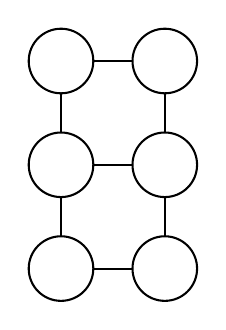
\begin{tikzpicture}[x=0.75pt,y=0.75pt,yscale=-1,xscale=1]
%uncomment if require: \path (0,166); %set diagram left start at 0, and has height of 166


% Text Node
\draw    (40, 30) circle [x radius= 15.56, y radius= 15.56]   ;
\draw (40,30) node   [align=left] {\begin{minipage}[lt]{13.600000000000001pt}\setlength\topsep{0pt}

\end{minipage}};
% Text Node
\draw    (90, 30) circle [x radius= 15.56, y radius= 15.56]   ;
\draw (90,30) node   [align=left] {\begin{minipage}[lt]{13.600000000000001pt}\setlength\topsep{0pt}

\end{minipage}};
% Text Node
\draw    (40, 80) circle [x radius= 15.56, y radius= 15.56]   ;
\draw (40,80) node   [align=left] {\begin{minipage}[lt]{13.600000000000001pt}\setlength\topsep{0pt}

\end{minipage}};
% Text Node
\draw    (90, 80) circle [x radius= 15.56, y radius= 15.56]   ;
\draw (90,80) node   [align=left] {\begin{minipage}[lt]{13.600000000000001pt}\setlength\topsep{0pt}

\end{minipage}};
% Text Node
\draw    (40, 130) circle [x radius= 15.56, y radius= 15.56]   ;
\draw (40,130) node   [align=left] {\begin{minipage}[lt]{13.600000000000001pt}\setlength\topsep{0pt}

\end{minipage}};
% Text Node
\draw    (90, 130) circle [x radius= 15.56, y radius= 15.56]   ;
\draw (90,130) node   [align=left] {\begin{minipage}[lt]{13.600000000000001pt}\setlength\topsep{0pt}

\end{minipage}};
% Connection
\draw    (55.56,30) -- (74.44,30) ;
% Connection
\draw    (40,45.56) -- (40,64.44) ;
% Connection
\draw    (90,45.56) -- (90,64.44) ;
% Connection
\draw    (40,95.56) -- (40,114.44) ;
% Connection
\draw    (90,95.56) -- (90,114.44) ;
% Connection
\draw    (55.56,130) -- (74.44,130) ;
% Connection
\draw    (55.56,80) -- (74.44,80) ;

\end{tikzpicture}